%% figures/fig_alpha_gain.tex  (2-panel, 2-column figure*)
%% (a) 모델별 mix throughput 이득 — spec-decode는 지배적이나 DeepSeek-R1 671B(MoE추론)만 음
%% (b) α vs gain 산점 (70 model×condition 셀) — break-even은 overhead로 이동

\begin{figure*}[t]
\centering
\begin{minipage}{0.46\textwidth}
\centering
\resizebox{\textwidth}{!}{%
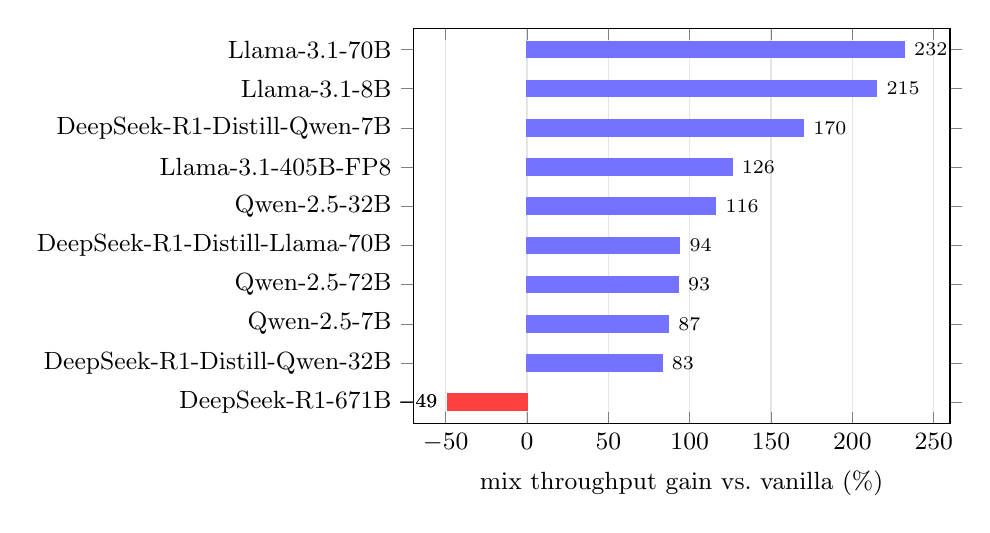
\begin{tikzpicture}
\begin{axis}[
  xbar, width=8.4cm, height=6.6cm,
  xlabel={mix throughput gain vs.\ vanilla (\%)},
  xmin=-70, xmax=260,
  symbolic y coords={DeepSeek-R1-671B,DeepSeek-R1-Distill-Qwen-32B,Qwen-2.5-7B,Qwen-2.5-72B,DeepSeek-R1-Distill-Llama-70B,Qwen-2.5-32B,Llama-3.1-405B-FP8,DeepSeek-R1-Distill-Qwen-7B,Llama-3.1-8B,Llama-3.1-70B},
  ytick=data, y dir=normal,
  nodes near coords, nodes near coords align={horizontal},
  every node near coord/.append style={font=\scriptsize},
  enlarge y limits=0.06, bar width=6pt, bar shift=0pt, font=\small,
  xmajorgrids, grid style={gray!20},
]
\addplot[fill=blue!55, draw=blue!55] coordinates {
(232,Llama-3.1-70B)(215,Llama-3.1-8B)(170,DeepSeek-R1-Distill-Qwen-7B)(126,Llama-3.1-405B-FP8)(116,Qwen-2.5-32B)(94,DeepSeek-R1-Distill-Llama-70B)(93,Qwen-2.5-72B)(87,Qwen-2.5-7B)(83,DeepSeek-R1-Distill-Qwen-32B)(-49,DeepSeek-R1-671B)};
\addplot[fill=red!75, draw=red!75] coordinates {(-49,DeepSeek-R1-671B)};
\end{axis}
\end{tikzpicture}}
\par\smallskip
{\footnotesize (a) 모델별 mix 이득. 8 dense/distill 모델은 $+83\!\sim\!+232\%$,
  MoE 추론 DeepSeek-R1 671B 만 $-49\%$.}
\end{minipage}\hfill
\begin{minipage}{0.50\textwidth}
\centering
\resizebox{\textwidth}{!}{%
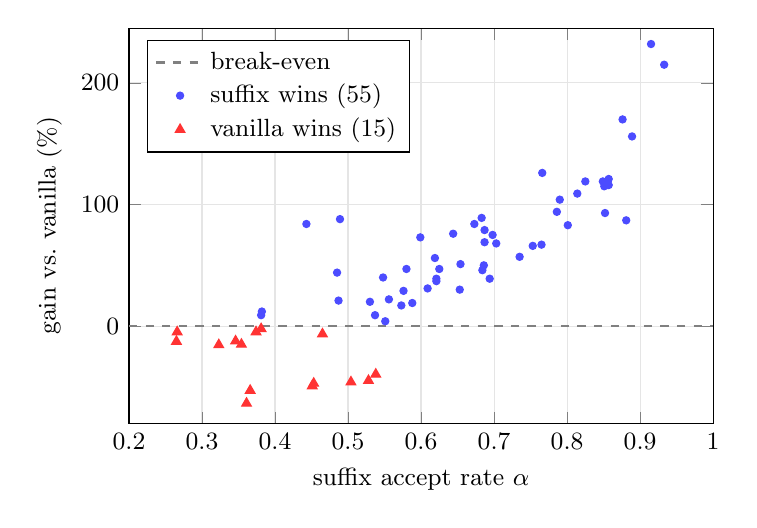
\begin{tikzpicture}
\begin{axis}[
  width=9.0cm, height=6.6cm,
  xlabel={suffix accept rate $\alpha$},
  ylabel={gain vs.\ vanilla (\%)},
  xmin=0.2, xmax=1.0, ymin=-80, ymax=245,
  grid=both, grid style={gray!20},
  legend pos=north west, legend cell align=left, font=\small,
]
\addplot[domain=0.2:1.0, dashed, gray, thick] {0};
\addplot[only marks, mark=*, mark size=1.3pt, blue!70] coordinates {
(0.786,94)(0.551,4)(0.573,17)(0.537,9)(0.588,19)(0.487,21)(0.381,9)(0.801,83)(0.621,37)(0.609,31)(0.576,29)(0.698,75)(0.580,47)(0.548,40)(0.876,170)(0.687,69)(0.687,79)(0.673,84)(0.825,119)(0.489,88)(0.703,68)(0.766,126)(0.735,57)(0.753,66)(0.653,30)(0.814,109)(0.443,84)(0.694,39)(0.915,232)(0.851,115)(0.857,121)(0.849,119)(0.889,156)(0.790,104)(0.765,67)(0.933,215)(0.654,51)(0.619,56)(0.625,47)(0.599,73)(0.644,76)(0.683,89)(0.857,116)(0.530,20)(0.556,22)(0.382,12)(0.277,209)(0.852,93)(0.686,50)(0.684,46)(0.485,44)(0.621,39)(0.881,87)};
\addplot[only marks, mark=triangle*, mark size=2.0pt, red!80] coordinates {
(0.504,-46.0)(0.528,-44.8)(0.453,-47.1)(0.361,-63.5)(0.366,-52.9)(0.538,-39.6)(0.451,-49.2)(0.346,-12.3)(0.354,-15.0)(0.374,-4.8)(0.323,-15.4)(0.265,-12.6)(0.381,-2.2)(0.465,-6.5)(0.266,-4.8)};
\legend{break-even, suffix wins (55), vanilla wins (15)}
\end{axis}
\end{tikzpicture}}
\par\smallskip
{\footnotesize (b) $\alpha$ vs.\ 이득(70 셀). vanilla-win(빨강)은 $\alpha\!\lesssim\!0.54$ 에 집중;
  DeepSeek-R1 671B 는 $\alpha\!\approx\!0.5$ 에서도 큰 손해($\because$ 큰 overhead).}
\end{minipage}
\caption{\textbf{spec-decode 는 지배적이나 불균일하다 (B200).}
  (a) 혼합 트래픽에서는 DeepSeek-R1 671B(MoE 추론)만 손해.
  (b) 단일 corpus 까지 보면 부호는 $\alpha$ 와 per-step overhead 의 경쟁으로 갈린다.}
\label{fig:alpha-gain}
\end{figure*}
